\documentclass[runningheads]{llncs}
\usepackage[T1]{fontenc}
\usepackage{graphicx}
\usepackage{subcaption}
\usepackage{pdfpages}
\usepackage{url}
\newcommand{\mybox}[1]{\vspace{0.5em}\hspace{-1.5em}\fbox{\parbox{\textwidth}{#1}}\vspace{0.5em}}
\newcommand{\myurl}[1]{{#1}}
\begin{document}
\title{GenAI 2 Years Later: Vibe Coding, Good or Bad?}
\author{
  Morten Heine Sørensen\inst{1} \and
  Mark Hissink Muller\inst{2}
}
\institute{
  Formalit, \email{mhs@formalit.dk} \and
  MHM Consult, \email{mark@mhmconsult.dk}
}
\maketitle
\begin{abstract}
A new era of GenAI arose late 2022, when ChatGPT3.5 was released.
Software developers soon prompted it to fix bugs and generate code.
But opinions varied; some predicted GenAI will replace developers, others discouraged the use of GenAI.
We suggested~\cite{Sorm2023} an approach to boost developer productivity and demonstrated it by a POC.

In the mean time, new models from various vendors emerged, and so did a set of {\em agentic\/} IDEs, which take automation to the next level. 
The latter further boost the approach we outlined back then. 

In this paper we show how this works, it is nowadays called {\em vibe coding\/}, by a combination of principles and examples coming partly from the original POC and partly from subsequent daily work experience.

\keywords{GenAI \and Agentic IDEs \and Programming \and Cursor \and ChatGPT}
\end{abstract}

\section{Introduction}\label{sec:introduction}
We present an approach to developing full stack applications with agentic IDE and LLM. The developer chats with the IDE, which annotates and forwards the request to the LLM, receives the response, which is also shown to the developer, and turns it into changes of files in the file system and commands in the terminal.
\begin{figure}[h]
    \centering
    \begin{subfigure}{0.38\textwidth}
        \centering
        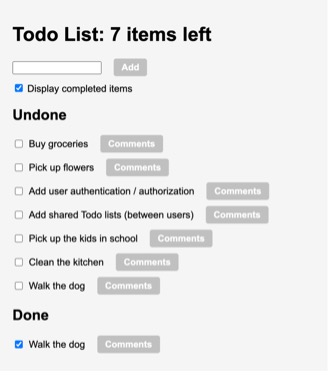
\includegraphics[width=\textwidth]{Pictures/Picture1.jpg}
    \end{subfigure}%
    \begin{subfigure}{0.38\textwidth}
        \centering
        
\includegraphics[width=\textwidth]{Pictures/Picture2.jpg}
    \end{subfigure}
    \caption{UI of the Todo-application}
    \label{fig:todo}
\end{figure}

\noindent The approach was originally tried out with ChatGPT in a POC where an application was developed from scratch up to production. The application manages todos~\cite{Freeman2013}, with the UI in Figure~\ref{fig:todo}.\footnote{See http://formalit.dk/portfolio.html for github links and presentation.}  The POC had these parts and steps:
\begin{itemize}
    \item UI built with React
    \item API built in Javascript running on Node.js
    \item Data layer with Postgres database
    \item UI hosted as Azure static web app
    \item API hosted as Azure app service
    \item Code in GitHub
    \item Automatic deployment on merge of each PR
\end{itemize}

\noindent In later projects in our daily work we have used {\em Cursor} as the agentic IDE~\cite{Cursor2023}. Some variants would be {\em Github CoPilot}~\cite{GitHubCopilot2023} or {\em Devin}~\cite{Devin2023}. In Cursor one can choose between various LLMs, we prefer GPT-4o~\cite{GPT402023}, some other options are some Claude~\cite{Claude2023} and Gemini~\cite{Gemini2023} models.

The remainder of the paper is organized as follows. We first explain the overall approach. Then follow sections with the detailed steps of the approach, drawing examples of the use of LLM from the POC and the use of agentic IDE from later experiences.  There is also a section with the details of the POC and one with details of later examples and the impact of the emerging agentic IDs.

\section{Overall Approach}
The approach can be briefly explained as follows. Imagine you are senior lead developer for a team of, say, five developers, excluding yourself. The developers are junior, medio or senior and front-end, back-end or full-stack developers.

Imagine you actively manage the team by providing functional requirements to each individual developer where work is organized in sprints. For the UI development it is in the form of screen shots (e.g., Figma) and user stories. For the DB layer, it will be by specifying tables and columns with primary and foreign keys. This carries over to the CRUD part of the API layer, which may also include, among others, validations, business logic, calculations and authentication and authorization.

Also imagine that the application has a skeleton which expresses how to deal consistently with common themes. For the UI, it will be how to manage state, where to place call-back handlers, how to call APIs, etc. For the API it will be, e.g., your selected separation into controller, service, and repo layers and how to manage ORM directly or by 3rd party libraries. The skeleton may come from you or the developers (or as the first step of the approach).

From this point on you delegate features to the developers. You review each pull request (PR) from each developer, possibly asking for revision of the code, e.g., to ensure consistency and completeness. After approving PRs, the API test and UI tests are automatically run and any errors are identified and communicated to the developers, who will fix them and start another cycle of the loop. The tests are extended by the developers to cover their new functionality.

Now imagine ChatGPT acting as each developer. The prompts correspond to the delegation to developers, and the generated answers make up the PRs. Finally realize that Cursor handles the communication with ChatGPT and implements the actual PRs by updating your files and issuing terminal commands for running the build, committing and pushing to github, etc.

The different steps of the approach are explained in the following sections.

\section{Set Up the Project}
This step is usually required only once for a range of sprints leading to one or more applications in the same company, so it does not have to be super-efficient. Nevertheless, ChatGPT can create a step by step instruction on how to set up the project and Cursor can actually do the steps.

\mybox{\textbf{Lesson 1:} ChatGPT can provide tutorials tailored to your application on how to accomplish any tasks. Cursor can actually do the steps on your laptop.}

\noindent The local development environment must be efficient to work with because it is crucial to have a fast loop of getting pull requests from ChatGPT, and letting cursor run the  UI and API tests and identify and fix issues.

 In the POC, we used a mixture of ChatGPT and \cite{Freeman2013} to provide basic setup of IDE and project files. There were a couple of issues with versions and dependencies, but they were not difficult to fix. We set up the code in a GitHub repository, which made it easy to backtrack when ChatGPT produced undesirable code. In other examples, we have used Cursor to set up Python projects handling existing and new dependencies very efficiently.

\mybox{\textbf{Lesson 2:} Set up the local development environment to efficiently support the iterations with ChatGPT and Cursor. It will be a one-time cost. Always begin with a GitHub repo to avoid loosing code by deletion or overwrites.}

\section{Get Started with Development}
Fowler\cite{Fowler2023} celebrates an approach, where you first communicate to ChatGPT an overall plan of steps that should be carried out before going into details.

The way we see it, this plan may reside in the mind of the team lead, who delegates parts to the individual developers without each of them necessarily knowing the entire plan.

For instance, for the POC, we could start with the code to generate the relevant database tables, then create the needed API, and finally create the UI.

\noindent In fact, we recommend following the three steps in this order (DB, API, UI) for one feature, and then repeat them for each new feature. There are many reasons why this iterative development is a good idea in conventional projects without ChatGPT, and they carry over to the new way of developing software with ChatGPT. For instance, it avoids the useless code Gewirtz\cite{Gewirtz2023a} experienced.

\mybox{\textbf{Lesson 3:} Split the development into sprints and user stories, like you would with a team of developers. Then proceed sprint by sprint, user story by user story, for the same reasons as you normally do.}

\mybox{\textbf{Lesson 4:} In Sprint 1, establish the fundamental architecture of the application, for instance a UI layer, an API layer, and the DB layer developed well enough to cover a small feature. The architecture should not only align to functional and non-functional requirements, but also to the team size and  experience.}

\section{Create the Data Model}
In a conventional project we would recommend developing a feature by doing the UI and API simultaneously, because each aspect helps to validate the other and together, they deliver a complete feature. The DB part can probably be done by the API developer, both are part of a typical back-end profile's capabilities.

With ChatGPT and a single development lead, the separate parts UI, API, DB are sequential, and we recommend doing them in the order DB, API, UI, since the UI needs the API, which needs the DB.

So, first generate the data model. Either you already know the entire data model, or you know only part of it. In any case, start with one or two example entities and create the DDL or migrations, depending on your preferred approach, to confirm that you get the expected results.

Some people recommend postponing the DB layer for various reasons. For instance, it is argued that the DB layer can change from relational to NoSql. Also, it is emphasized that it is important to solicit quick feedback from product management, which suggests emphasizing the UI.

However, in our experience most applications have a data model, relational or otherwise, and understanding this model is the key to have a solid basis for the entire application.

\mybox{\textbf{Lesson 5:} Except for mock-ups, UI experimentation and hobby projects, most sprints should start by implementing the data model of the feature.}

\section{Create the API}
Having created the necessary tables for a feature, you can proceed with the API.
You should first generate a small part, verify what ChatGPT provides and make sure that it meets expectations. Although it is impressive how accurate and
correct ChatGPT's answers often are, also in our experience, they are not flawless. Mistakes encountered include basic oversights (for which it always politely apologizes), but occasionally also more fundamental flaws that indicate that it completely misses the point.

\mybox{\textbf{Lesson 6:} ChatGPT's answers should be evaluated like they come from another (sometimes less experienced) person, rather than from a flawless machine. The human developer remains liable.}

\noindent If you are not content with the results that ChatGPT provides, it is often advisable to iterate to get what you want. If, however, you are confident that the code is correctly structured, you could go for the overall thing in a second round after the initial sprint.

Also, if you are delivering to a company that has policies for how the code should be structured, you can ask ChatGPT that the code be so structured.

For instance, do you have multiple layers with controller, service, and repo, or less than that. In general, keep things as simple as possible. The fewer moving parts and the fewer proprietary add-ons that ChatGPT has no knowledge about, the easier it will be for ChatGPT to get it right. Besides, you can always get ChatGPT to rewrite the 
files later if you decide.

Remember the API is not just happy scenario, so provide instructions about error handling, return codes, etc. For instance, in the POC, the API server could initially crash when there was some issue. So we asked ChatGPT to wrap each call in a try catch, and return 200 or 500 depending on whether an error was encountered or not. We should note that on several other occasions, ChatGPT actually suggested that error handling should be part of the implementation and provided examples of how to do it.

\mybox{\textbf{Lesson 7:} When starting the API, get a simple server running with a simple example and make sure you are happy with it to some level of maturity. There may be some production hardening missing that can be covered later, but the basic structure should be correct and satisfactory.}

\section{Create the UI}
Having established DB and API for the first sprint, proceed to the UI. Initially this was where we saw the largest difference working with ChatGPT, compared to the conventional approach.

With a developer you will typically show a screen shot of some sort, or maybe Figma wireframes produced by product management, accompanied by some explanations.
But early ChatGPT did not support upload of files, so we relied on only explanations. This made it more difficult to explain details like horizontal and vertical layout, and added to the possibilities for incorrect interpretation, leading to incorrect or suboptimal results. Even with later versions that support file upload, there is a limit to the complexity of the UI in terms of the number of controls and fragments that ChatGPT can generate HTML and CSS for.

Therefore, we should divide a page with multiple controls and fragments into more manageable parts and proceed part by part in an iterative way.
This process helps keep to the code and the development process – here meaning the interaction with ChatGPT – under control. You get small parts, which can easily be validated and tested. In other words, we do not end up with legacy code, contrary to the claim of Loukides\cite{Loukides2023}.

\mybox{\textbf{Lesson 8:} When working with ChatGPT on User Interface, ask first for a simple version. Then add remaining controls one by one or in small groups.}

\noindent We will later discuss how we can scale the development of UI to a more efficient process where the UI is explained in a semi-formal way.

\section{Intermezzo 1: the POC in Detail}
In \cite{Freeman2013} the development of the Todo application proceeds from UI to API (contrary to our recommendation, but the book is about React, so it makes sense). Let's follow that path and see how ChatGPT works it out. In what follows, "SC $n$" refers to the screenshot $n$ in the appendix, which will be made available online.

We start with the standard dummy React application npx create-react-app todo. Next, we ask ChatGPT for contents for the dummy files (SC 1). We want a single page with an input field and an Add button and the list of todos. The todos are for now just kept in local storage of the browser.

When you ask ChatGPT to generate code it will often give you examples and leave to you to complete the details. However, it is much faster if ChatGPT simply does it all. So, we ask for full contents of the files. With Cursor, this is less of an issue, because it updates the files directly in the file system.

\mybox{\textbf{Lesson 9:} Ask for full contents of files. It speeds up the process.}

We get back a list of the 5 affected files (SC 2) and then the contents of each file (SC 3-4) as well as some free advice about how wo run the application.

Sometimes there can be slight imprecisions in ChatGPT's responses. For instance, about the name of entities, file locations, etc. That's why it's good to have a working dummy application where files are correctly named and stored in locations that are consistent.

\mybox{\textbf{Lesson 10:} When starting the interaction with ChatGPT, have a dummy application working.}
Next, we want to indicate whether todos are done with check marks (SC 5). ChatGPT responds with the relevant changes to 4 files (SC 6-9).
    
We confirm the code is working and move on to the next missing part, which is splitting the todo list into two lists: done and not done (SC 10).
ChatGPT responds with the list of affected files and the actual contents (SC 11-13).
  
We are then ready for the last part, which is a check mark indicating whether completed todos should be displayed (SC 14), and ChatGPT responds with the changes (SC 15).

The application (focused on UI) now has most of what is shown in Section~\ref{sec:introduction}, except the Comments page, the
styling, and a few details. Now we move on with the API and ask for a server offering the needed end points and just keeping todos in memory (SC 16).
ChatGPT responds wit a new file with the API and modifies one existing file (SC 17-18).

We ask ChatGPT how to test the end points (SC 19) and it provide some curl commands (SC 20).
After we try out the end points and confirm they are working we can make ask that the UI uses them(SC 21), and ChatGPT shows how to change the UI to use them (SC 22-23).

As mentioned, sometimes ChatGPT will generate code that does not work. In many cases it is because of small details like not naming paths in json correctly (because of lack of context). In general, ChatGPT is pretty good at helping with the issues.

In this case we have a CORS issue, which we ask for help with (SC 24), and we get some advice (SC 25). The advice turns out to work. In general, such advice should be confirmed by checking with other sources. Although, code is contributed by ChatGPT, you should see yourself as liable for it. See~\cite{Gewirtz2023c} for more on this aspect and~\cite{Gewirtz2023b} for questions about copyright regarding the code. Also notice that confidential code or information should not be shared with ChatGPT as observed in~\cite{Fowler2023}, unless you have a private model.
  
\mybox{\textbf{Lesson 11:} ChatGPT may generate code with issues for various reasons, e.g., because we did not ask explicitly to avoid them or because it made an interpretation that is incorrect in our context. In such cases, simply ask for help; most of the time it will it able to (help) resolve the problem.}

\noindent At this point, repeated testing reveals some new errors, ChatGPT replies with new versions where the errors are solved, and the ping-pong game continues for a little while until the code eventually works. Again, the trick is to get ChatGPT to do the work and keep providing the updated component in full, rather than to provide instructions for the developer to address these himself.

\mybox{\textbf{Lesson 12:} As mentioned, ChatGPT may generate code with errors but getting it to fix them is quicker than writing the code yourself, which may also introduce errors that may take time to find and resolve.}

\noindent Interestingly, at the end, the todo items are back in single list, rather than two different for done and undone. ChatGPT lost some context along the way in the new issues, as others have reported, and we had to get it back on track. Also, we had to instruct it that the API should be called to mark todo items done or not done.

\mybox{\textbf{Lesson 13:} ChatGPT may generate code with problems that were solved earlier in the dialog. You need to test what it returns at every step and ask errors to be fixed.}

\noindent We will say more about automatic testing later. It's finally time to get the DB layer done. We ask for SQL to create the table and for the API to be rewritten to use the DB rather than keeping todos in memory (SC 26), and we get both from ChatGPT (SC 27-28).

\noindent Then follows some more ping-pong about the user which the API should connect to the DB with.

\mybox{\textbf{Lesson 14:} Be as precise as you can in stating what you need from ChatGPT. Whenever you omit details, ChatGPT may do something else than you expect.}

\noindent Not long after this we have an application that works with all three layers. However, there are still many details
missing before the application is appropriate for production. For instance, the server code is in one big file which does not scale for a bigger API. Also, there is no error handling. We return to these and other issues later.

\mybox{\textbf{Lesson 15:} If ChatGPT is lacking context, it may make assumptions instead of asking for clarifications. You can circumvent this by explicitly directing it initially to ask clarifications.}

\section{Create the Styling}
If the DB layer is the nitty-gritty details below the API, the styling is the nitty-gritty details above the UI.
Explaining styling to ChatGPT is even worse than explaining the basic layout of pages.

 At the time, there were various offerings that could generate artifacts from drawings or even Figmas. We tried out one with not the results we needed. For instance, it was not possible to generate React code.

Instead, we tried to get ChatGPT to generate HTML and CSS for some complex examlpes. it correctly used an HTML grid and got the basic layout right, but adjusting the details turned out to be impossible after 2-3 iterations. At this point we reverted to classical techniques and studied HTML and CSS documentation and manually did the needed adjustments.

\mybox{\textbf{Lesson 16:} Sometimes, several iterations do not bring you closer to a solution. In these cases, revert to classical techniques, like Googling, Stack Overflow, YouTube demos, reading the documentation, etc.}

\noindent Nevertheless, notice that you can request that controls be used from standard libraries such as material-ui1. 
However, also notice that ChatGPT is always trained on material up to a certain date in the past, so it may prefer approaches that are not fully up to date.
For instance, In the POC, when we later created a basic application based on Next.js, it was expecting a file
 structure based on the classical router with the pages directory. In contrast, the default option when creating Next.js applications uses the App router.

\mybox{\textbf{Lesson 17:} ChatGPT does not know about knowledge published after some date in the past.}

\noindent Anyway, in the meantime, several approaches have evolved such as {\em Locofy.ai}~\cite{LocofyAI2023}, {\em Anima}~\cite{Anima2023}, {\em Builder.io}~\cite{BuilderIO2023}.

\section{Create the Tests}
As mentioned, ChatGPT – like most developers – generates code with errors, even errors that were previously fixed.
The most efficient approach to dealing with these is to have two slim test suites, one that tests the API and one that tests the UI.
For the POC, the UI test was produced with Puppeteer. It has these steps:
\begin{enumerate}
    \item Open browser and go to main page
    \item Click Show completed todos
    \item Type into the item input field
    \item Click the "Add" button
    \item Confirm the new item is there
    \item Click the new item's check mark
    \item Check the new item is now in the done list
    \item Deleting the new item using the API
\end{enumerate}

\noindent When adding new functionality from ChatGPT we check locally that the UI test runs before merging the pull request. We also manually check the new feature works and add a UI test for it. We prefer to first check it manually, so that if the generated automatic test fails, we know the problem is with the test.

The API test was a sequence of API calls in code using axios (a HTTP client library) imitating a UI interaction. Again, the test ends by deleting the data it has added using the API.

\mybox{\textbf{Lesson 18:} ChatGPT generates several errors. It is valuable to have a slim UI test and API test that can be run locally before merging pull requests.}

\noindent We do not bother to mock database or service layer. Since we have the development environment running locally, we can rely on it as long as the tests:
\begin{itemize}
    \item Do not make any assumptions about the condition of the database on entry.
    \item Leave the database in the same condition on exit as it was in on entry.
\end{itemize}

\mybox{\textbf{Lesson 19:} By keeping the tests slim, lightweight, and direct, they do not need to be time consuming and can be a good way of testing pull requests from ChatGPT.}

\noindent The tests were written manually, because we wanted to make sure the code from ChatGPT did what we asked. Some people prefer to let ChatGPT generate the tests, but we see a risk that when ChatGPT gets something wrong in code, it will get the same thing wrong in tests. Indeed, errors were frequently about aspects that were not sufficiently well communicated, e.g., field names.

Nevertheless, we are open to the approach that you start by having ChatGPT create the tests and review that they capture what you want.

\section{Intermezzo 2: Cursor as a Game Changer}
In retrospect, the ping pong between ChatGPT and the user in the original POC was rather tedious, consisting of prompting for code, copy/pasting the code into the classic IDE, running the UI and API test, seeing an error, prompting it to ChatGPT, getting an attempted code fix, etc. 

Today with agentic IDE, we can prompt Cursor to generate the code needed for a new feature, update the relevant files, run the UI and API tests and not come back until the tests actually work. Sometimes it will go into an indefinite loop of trying the same failing thing repeatedly, in which case we simple stop the process and take over.

Similarly, we can let Cursor manage the GitHub activity, i.e. add, commit and push changes. It can also create branches and create and merge PRs. In general, anything you can accomplish from the command line, you can let Cursor do.

This is a little thought-provoking, because how can we be sure it does not do things we do not want it to do, e.g. in the case of prompt injections to the model.
It is a setting in Cursor whether it can automatically execute commands, and when the setting is enabled, it is possible to specify commands that should be whitelisted or blacklisted.

\mybox{\textbf{Lesson 20:} Delegate code build, regression test, GitHub operations, and the like to Cursor, but review every single PR before merge. If you accept auto execution, specify whitelist commands}

We also briefly review three recent applications of ChatGPT and Cursor in our daily work.

1. We worked on a short part-time assignment as an IT-architect in the fraud section of a financial institution and defined a certain pattern to be recognized by KYC Code. We wanted to confirm that the pattern captured real life examples from production and got 1 Gb data extract. We had no development environment at hand on the handed out lap top, but it had Windows PowerShell installed, in which we never coded a single line. We used ChatGPT to write a Windows Powershell script that reads the data and checks the pattern and tested the code carefully. The work was completed in a few hours on one day. It turned out that 95\% of transactions were correctly identified.

2. Working on a machine learning project to identify active peptide sequences. We first used ChatGPT and vanilla Python to leverage Michael Nielsen's classical code for neural networks, but then switched to Cursor and used PyTorch to quickly code relevant models. Cursor got the Python evironment with needed dependencies installed in a few minutes and made it possible to code new models in no time.

3. Working on a tutorial for an AI Conference. Using Cursor to write the LaTeX code for the tutorial and let it manage the GitHub operations. Everything it writes, we have written in other papers or books, but is is just way faster to have it write the LaTeX code.

\section{Refactor Out Common Parts}
When you ask ChatGPT to generate some code, it will try to satisfy your requirements, but in many cases, it will refrain from satisfying your untold requirements, even if you regard them as common sense.

To be fair, when it generates some code, it will sometimes tell you that this is just an example, and you also need to take into account some list of considerations. But at the end of the day, you cannot assume it satisfies non-functional requirements that you do not mention.

An obvious example is when the same code occurs in multiple places. In this case we want to factor it out.

For instance, in the POC we added the possibility to have some fields of the todo encrypted in the database, so that developers cannot see the contents of the fields when they access the database.

The code to encrypt when storing and decrypt when fetching should not be replicated to the handler of each end point. There should rather be utility functions that are called from the API endpoints handlers:
 
You can handle these requirements up front when asking code to be generated or refactor along the way by explaining to ChatGPT the current files and their contents and the required refactoring.

\mybox{\textbf{Lesson 21:} As you review PRs from ChatGPT, keep an eye on parts of the code that should be refactored. Do the refactoring yourself or ask ChatGPT to do it.}

\noindent In general, we want to limit refactoring to a reasonable limit and only allow it when it has a tangible result and good balance between effort and benefit not based solely on speculation.

But some refactoring just has to be done. Like having significant chunks of code that is replicated verbatim in many methods pulled out to a method.

\section{Design The File Structure}
When you design your application with ChatGPT there are typically two different approaches:
\begin{itemize}
    \item You did this many times and have a clear idea about the major design and architecture choices.
    \item You are doing this in an exploratory manner.
\end{itemize}

\noindent Both approaches have their merits. If you work in the explanatory way, you should expect to do refactoring along the way. ChatGPT can provide advice on the structure and even generate the files. 

Have a clear structure for the files of your application in mind from the beginning and communicate it to ChatGPT in your prompts, or be prepared that you or ChatGPT should refactor the code along the way to replace a single file by a set of files each of which covers a feature.

\noindent Similarly, be prepared that as more complexity arrives, a single layer may be split into several layers, e.g., for the API as service, controller, repo, etc.

\mybox{\textbf{Lesson 22:} You are responsible for ensuring that the file structure of the application is manageable. Define it from the outset or refactor it (with the help of ChatGPT) along the way.}

\section{Keep The Code Under Control}
As mentioned, you should be prepared to refactor. What was said in the preceding section was about splitting large files into smaller more manageable files, e.g., 
splitting a single file with the handlers for all end points into separate files grouped by entity or entity groups.

Also, we have mentioned that every response from ChatGPT should be seen as a pull request. That way no code ever enters the code repository without some sanity check. You don't need to read every single line, but you need to gain confidence that the code follows the philosophy and guidelines that you are trying to enforce. What we can add to this is that the code should be structurally consistent. This means that how different kinds of functionality or logic is structured or organized should be the same from feature to feature.
  
 For instance, in the POC, the page fragments were initially classes. However, when we added the page for adding comments on todos, we introduced version 6.14.1 of react-router-dom and had to make use of the useParams and useNavigate hooks for retrieving the URL parameters and for navigation, respectively. And this led to some classes being reformulated as functions. In this case, it is preferable that all the components are functions.

The reason ChatGPT got us into the classes formulation in the first place may be that this was the most widespread method during the period of documents that ChatGPT has 
been trained with.

\mybox{\textbf{Lesson 23:} Keep the code consistent. ChatGPT may change structure of the code it generates when new requirements from you become clear. You should refactor the previously generated code (make ChatGPT do it) when this happens. Consider code measurement tooling at the end of the project to confirm and document consistency.}

\noindent It is claimed in~\cite{Gamage2023} regarding the code generated by ChatGPT that "For all practical purposes, it's 'legacy code,' even if it's only a few minutes old." As hinted at earlier, this does not apply to the approach described here:
\begin{enumerate}
    \item Developers may leave you and are not there to explain their code. ChatGPT and related technologies are here to stay and will improve over time.
    \item You must review the code from ChatGPT and adopt it as your own code. So long as you are there, it's not legacy.
    \item Code generated in Cursor is commented, and the comments give a very good idea about the code.
\end{enumerate}    

\mybox{\textbf{Lesson 24:} See the code by ChatGPT as your code. You must be able to account for it. That way it has same value as code developed by you or your developers.}

\section{Mature for Production}
So, you have your code generated by ChatGPT and it does what you asked. The UI tests run, the API tests run, all good. But are you ready for production?
If you are an experienced developer, you know many things are missing. For instance, you may need a penetration test to ensure that you did everything to correctly handle 
security-related HTTP-headers, SQL injection attacks, cross-site scripting etc.

Actually, you can ask ChatGPT what is required from, say, an API before it is mature for production, and it will provide a checklist, which is a good starting point that can be elaborated upon as needed (see SC 16-17 in the appendix). Such responses should be checked with alternative sources.

\mybox{\textbf{Lesson 25:} The code that you get from ChatGPT may not be ready for production, but it can help you understand what needs to be checked and how, and which changes are needed as a result of the checks.}

\section{Set Up The Prod Environment}

Like with the development environment, we eventually need a production environment.

For the POC, we used Azure Postgres for the database layer. For the UI and the API, we initially used Azure App service. For the UI, upload took ages and there were some issues getting it to work. After a while we backtracked and looked for demos of how to deploy a React application on Azure and changed to Azure static web app, which ran much smoother.

We need some additional DevOps work. For instance, as mentioned, for the POC we set up a GitHub repository and had automatic deploy to the environment when there are commits to the branch.

Depending on your organizational setup, number of applications to develop, etc. you may find it desirable to script provisioning of your environments as is often done.

\section{Scale With Formalism}

Once you start doing multiple applications with ChatGPT, it becomes natural to optimize the communication.

One interesting possibility is that you can train ChatGPT with training material yourself. That is, you can give examples of what prompts you provide and at the same time provide the desired answer.

\noindent This can be used to train it to deal with formal specifications of UI. For instance, you provide a text representation of a UI by listing all the components of a page including alignment margins etc. and show the HTML or React code you expect.

We have already pursued this approach some way but leave as future work to report on it in detail.

\mybox{\textbf{Lesson 26:} Formalize your communication with ChatGPT with initial training. That way the communication can hopefully be way more efficient and less ambiguous.}
  
\section{Conclusion}
We have outlined an approach to developing mature, production-ready, maintainable full stack applications from scratch with ChatGPT and Cursor. Based on our examples we estimate the productivity improvement to be a factor between 2 and 5.

The method does not work out of the box, you must adopt various practices. Most importantly, you should work the same way as you do today with developers.
\begin{itemize}
    \item Create the architecture and features in sprints.
    \item Regard the code you get as pull requests that you should review.
    \item Implement lightweight regression testing for UI and API to confirm that refactoring and adding functionality does not break anything.
    \item Request refactoring along the way to turn duplicated code into methods and to implement other patterns that you observe the need for in the pull request reviews.
\end{itemize}

\noindent There are some limitations to the approach. For instance, ChatGPT may be periodically unavailable, the free versions have some limitations, and the knowledge base only goes to some point in the past. Also, Cursor sometimes crashes or loses connection with the file system. In practice we have so far not found these limitations to severely restrict the benefits.

Our hands-on experiments suggest that Cursor and ChatGPT, guided the right way, can contribute working code, identify relevant libraries and frameworks, fix bugs, suggest methods to mature and secure the application, and contribute in many other ways that save time and money, and improve quality and time-to-market.

ChatGPT and Cursoer can make mistakes, but so can developers, professors, and textbooks. When you receive advice that you cannot confirm satisfactorily yourself, it is always good to double check with an alternative authoritative source. At the end of the day, we think of ChatGPT as a developer that read all the relevant documents and pieces of code that exist for that language in question and gives the best answer to your question at hand. In most cases, ChatGPT and Cursor can do things faster than you can. Whenever getting caught up in anything that seems routine, ask yourself this question: Shouldn't I get ChatGPT to do this?

In short, vibe coding with ChatGPT and Cursor can be good.

\bibliography{references}
\bibliographystyle{plain} 

\newpage
\section*{Appendix}
\includepdf[pages=-]{Pictures/Screenshots.pdf}
\end{document}
